% -*- coding: utf-8 -*-
%-------------------------designed by zcf--------------
\documentclass[UTF8,a4paper,10pt,fontset=none]{ctexart}
\usepackage[left=3.17cm, right=3.17cm, top=2.74cm, bottom=2.74cm]{geometry}
\usepackage{amsmath}
\usepackage{graphicx,subfig}
\graphicspath{{record_Lab1/images/}}  % 练习截图
\usepackage{float}
\usepackage{cite}
\usepackage{caption}
\usepackage{enumerate}
\usepackage{booktabs} %表格
\usepackage{multirow}
\newcommand{\tabincell}[2]{\begin{tabular}{@{}#1@{}}#2\end{tabular}}  %表格强制换行
%-------------------------字体设置--------------
% \usepackage{times} 
\usepackage{ctex}
% 中文字体按系统自动选择，需用 XeLaTeX 编译。每种字体依次尝试：
%   macOS 系统字体 -> Noto CJK / 思源 -> Windows 系统字体 -> TeX Live 自带 Fandol。
% 没有粗体的字体（如 SimSun、KaiTi、Fandol 楷体）用伪粗体代替。
% 需要在不同机器上得到完全相同的排版时，取消下一行注释，强制使用 Fandol。
\newif\iflabfandol
% \labfandoltrue
\makeatletter
% \lab@cand{角色}{字体名或文件名}{fontspec 选项}：角色尚未选定且字体存在时选用。
\newcommand\lab@cand[3]{%
  \expandafter\ifx\csname lab@#1@font\endcsname\relax
    \IfFontExistsTF{#2}{\@namedef{lab@#1@font}{#2}\@namedef{lab@#1@opt}{#3}}{}%
  \fi}
\newcommand\lab@fandol{%
  \lab@cand{song}{FandolSong-Regular.otf}{BoldFont=FandolSong-Bold.otf}%
  \lab@cand{hei}{FandolHei-Regular.otf}{BoldFont=FandolHei-Bold.otf}%
  \lab@cand{kai}{FandolKai-Regular.otf}{AutoFakeBold=2.5}%
  \lab@cand{fang}{FandolFang-Regular.otf}{AutoFakeBold=2.5}}
\iflabfandol\lab@fandol\fi
% 宋体（正文）
\lab@cand{song}{Songti SC}{BoldFont=* Bold}
\lab@cand{song}{Noto Serif CJK SC}{}
\lab@cand{song}{Source Han Serif SC}{}
\lab@cand{song}{SimSun}{AutoFakeBold=2.5}
% 黑体（无衬线）
\lab@cand{hei}{PingFang SC}{BoldFont=* Semibold}
\lab@cand{hei}{Noto Sans CJK SC}{}
\lab@cand{hei}{Source Han Sans SC}{}
\lab@cand{hei}{Microsoft YaHei}{}
\lab@cand{hei}{SimHei}{AutoFakeBold=2.5}
% 楷体
\lab@cand{kai}{Kaiti SC}{BoldFont=* Bold}
\lab@cand{kai}{STKaiti}{AutoFakeBold=2.5}
\lab@cand{kai}{KaiTi}{AutoFakeBold=2.5}
\lab@cand{kai}{AR PL UKai CN}{AutoFakeBold=2.5}
% 仿宋
\lab@cand{fang}{STFangsong}{AutoFakeBold=2.5}
\lab@cand{fang}{FangSong}{AutoFakeBold=2.5}
\lab@fandol
% \lab@use{命令}{角色}：用选定的字体和选项展开字体设置命令。
\newcommand\lab@use[2]{%
  \edef\lab@tmp{\noexpand#1[\csname lab@#2@opt\endcsname]{\csname lab@#2@font\endcsname}}%
  \lab@tmp}
\lab@use\setCJKmainfont{song}
\lab@use\setCJKsansfont{hei}
\lab@use\setCJKmonofont{hei}
\lab@use{\setCJKfamilyfont{zhsong}}{song}
\lab@use{\setCJKfamilyfont{zhhei}}{hei}
\lab@use{\setCJKfamilyfont{zhkai}}{kai}
\lab@use{\setCJKfamilyfont{zhfs}}{fang}
\typeout{Lab report CJK fonts: song=\lab@song@font, hei=\lab@hei@font,
  kai=\lab@kai@font, fang=\lab@fang@font}
\makeatother
\providecommand*\songti{}\renewcommand*\songti{\CJKfamily{zhsong}}
\providecommand*\heiti{}\renewcommand*\heiti{\CJKfamily{zhhei}}
\providecommand*\kaishu{}\renewcommand*\kaishu{\CJKfamily{zhkai}}
\providecommand*\fangsong{}\renewcommand*\fangsong{\CJKfamily{zhfs}}
\newcommand{\yihao}{\fontsize{26pt}{36pt}\selectfont}           % 一号, 1.4 倍行距
\newcommand{\erhao}{\fontsize{22pt}{28pt}\selectfont}          % 二号, 1.25倍行距
\newcommand{\xiaoer}{\fontsize{18pt}{18pt}\selectfont}          % 小二, 单倍行距
\newcommand{\sanhao}{\fontsize{16pt}{24pt}\selectfont}  %三号字
\newcommand{\xiaosan}{\fontsize{15pt}{22pt}\selectfont}        % 小三, 1.5倍行距
\newcommand{\sihao}{\fontsize{14pt}{21pt}\selectfont}            % 四号, 1.5 倍行距
\newcommand{\banxiaosi}{\fontsize{13pt}{19.5pt}\selectfont}    % 半小四, 1.5倍行距
\newcommand{\xiaosi}{\fontsize{12pt}{18pt}\selectfont}            % 小四, 1.5倍行距
\newcommand{\dawuhao}{\fontsize{11pt}{11pt}\selectfont}       % 大五号, 单倍行距
\newcommand{\wuhao}{\fontsize{10.5pt}{15.75pt}\selectfont}    % 五号, 单倍行距
%-------------------------章节名----------------
\usepackage{ctexcap} 
\CTEXsetup[name={,、},number={ \chinese{section}}]{section}
\CTEXsetup[name={（,）},number={\chinese{subsection}}]{subsection}
\CTEXsetup[name={,.},number={\arabic{subsubsection}}]{subsubsection}
%-------------------------页眉页脚--------------
\usepackage{fancyhdr}
\pagestyle{fancy}
\lhead{\kaishu \leftmark}
% \chead{}
\rhead{\kaishu 操作系统}%加粗\bfseries
\lfoot{}
\cfoot{\thepage}
\rfoot{}
\renewcommand{\headrulewidth}{0.1pt}  
\renewcommand{\footrulewidth}{0pt}%去掉横线
\newcommand{\HRule}{\rule{\linewidth}{0.5mm}}%标题横线
\newcommand{\HRulegrossa}{\rule{\linewidth}{1.2mm}}
%-----------------------伪代码------------------
\usepackage{algorithm}  
\usepackage{algorithmicx}  
\usepackage{algpseudocode}  
\floatname{algorithm}{Algorithm}  
\renewcommand{\algorithmicrequire}{\textbf{Input:}}  
\renewcommand{\algorithmicensure}{\textbf{Output:}} 
\usepackage{lipsum}  
\makeatletter
\newenvironment{breakablealgorithm}
  {% \begin{breakablealgorithm}
  \begin{center}
     \refstepcounter{algorithm}% New algorithm
     \hrule height.8pt depth0pt \kern2pt% \@fs@pre for \@fs@ruled
     \renewcommand{\caption}[2][\relax]{% Make a new \caption
      {\raggedright\textbf{\ALG@name~\thealgorithm} ##2\par}%
      \ifx\relax##1\relax % #1 is \relax
         \addcontentsline{loa}{algorithm}{\protect\numberline{\thealgorithm}##2}%
      \else % #1 is not \relax
         \addcontentsline{loa}{algorithm}{\protect\numberline{\thealgorithm}##1}%
      \fi
      \kern2pt\hrule\kern2pt
     }
  }{% \end{breakablealgorithm}
     \kern2pt\hrule\relax% \@fs@post for \@fs@ruled
  \end{center}
  }
\makeatother
%------------------------代码-------------------
\usepackage{xcolor} 
\usepackage{listings} 
\lstset{
breaklines,%自动换行
basicstyle=\small,
escapeinside=``,
keywordstyle=\color{ blue!70} \bfseries,
commentstyle=\color{red!50!green!50!blue!50},% 
stringstyle=\ttfamily,% 
extendedchars=false,% 
linewidth=\textwidth,% 
numbers=left,% 
numberstyle=\tiny \color{blue!50},% 
frame=trbl% 
rulesepcolor= \color{ red!20!green!20!blue!20} 
}
%------------超链接----------
\usepackage[colorlinks,linkcolor=black,anchorcolor=blue]{hyperref}
%------------------------TODO-------------------
\usepackage{enumitem,amssymb}
\newlist{todolist}{itemize}{2}
\setlist[todolist]{label=$\square$}
% for check symbol 
\usepackage{pifont}
\newcommand{\cmark}{\ding{51}}%
\newcommand{\xmark}{\ding{55}}%
\newcommand{\done}{\rlap{$\square$}{\raisebox{2pt}{\large\hspace{1pt}\cmark}}\hspace{-2.5pt}}
\newcommand{\wontfix}{\rlap{$\square$}{\large\hspace{1pt}\xmark}}
%------------------------水印-------------------
\usepackage{tikz}
\usepackage{xcolor}
\usepackage{eso-pic}

\newcommand{\watermark}[3]{\AddToShipoutPictureBG{
\parbox[b][\paperheight]{\paperwidth}{
\vfill%
\centering%
\tikz[remember picture, overlay]%
  \node [rotate = #1, scale = #2] at (current page.center)%
    {\textcolor{gray!80!cyan!30!magenta!30}{#3}};
\vfill}}}



%———————————————————————————————————————————正文———————————————————————————————————————————————
%----------------------------------------------
\begin{document}
\begin{titlepage}
    \begin{center}
    
\includegraphics[width=0.8\textwidth]{NKU.png}\\[1cm]    
    {\Huge \kaishu{\textbf{南\ \ \ \ \ \ 开\ \ \ \ \ \ 大\ \ \ \ \ \ 学}} }\\[0.9cm]
    {\huge \kaishu{\textbf{计\ \ 算\ \ 机\ \ 学\ \ 院}}}\\[0.5cm]
    {\Large \textbf{操作系统}}\\[0.8cm]
    \HRule \\[0.9cm]
    \vspace{0.4cm}
    \HRule \\[2.0cm]
    \centering
    {\LARGE \kaishu{白景仁\ \ 陈彦兴\ \ 何闻硕}}\\[0.5cm]
    {\LARGE \kaishu{年级\ :\ 2026级}}\\[0.5cm]
    {\LARGE \kaishu{专业\ :\ 计算机科学与技术}}\\[0.5cm]
    {\LARGE \kaishu{指导教师\ : 袁晓洁\ \ 李浩然}}\\[0.5cm]
    \vfill
    {\Large \today}
    \end{center}
\end{titlepage}
%-------------摘------要--------------
\newpage
\thispagestyle{empty}
\renewcommand{\abstractname}{\kaishu \sihao \textbf{摘要}}
    \begin{abstract}
        \noindent  %顶格
        \textbf{\\\ 关键字：}\textbf{} \\\ \\\
    \end{abstract}
%----------------------------------------------------------------
\tableofcontents
%----------------------------------------------------------------
\newpage
\watermark{60}{10}{NKU}
\setcounter{page}{1}
\section{实验基本信息与小组分工}
\subsection{实验名称与完成日期}
Lab1：最小可执行内核。完成日期：10月12日。
\begin{itemize}
    \item 白景仁：练习一、补充观察。
    \item 陈彦兴：练习二。
    \item 何闻硕：练习二、实验总结。
\end{itemize}

\section{实验目的}
\begin{enumerate}
    \item 阅读 \texttt{kern/init/entry.S}，理解内核入口如何为 C 代码准备运行环境。
    \item 用 GDB 跟踪 QEMU 模拟的 RISC-V 从加电到执行内核第一条指令的过程，
          弄清复位代码、OpenSBI 和内核之间的交接方式。
    \item 熟悉 QEMU 与 GDB 联合调试裸机程序的基本方法。
    \item 练习用 AI 辅助阅读代码和分析调试现象，并用实际输出核对 AI 的解释。
\end{enumerate}

\section{实验环境}
\subsection{硬件、操作系统与工具链}
\begin{table}[H]
   \centering
   \begin{tabular}{|c|c|}
        \hline
        软件 & 版本 \\
        \hline
        riscv64-unknown-elf-gcc & 16.2.0 \\
        qemu-system-riscv64 & 11.1.2 \\
        \hline
    \end{tabular}
\end{table}

\subsection{GDB 跟踪所用环境}
上表是本报告中编译和运行结果所用的环境。练习一、练习二的 GDB 截图和日志是在小组另一台机器上
采集的，环境如下：
\begin{table}[H]
    \centering
    \begin{tabular}{|c|c|}
        \hline
        项目 & 配置 \\
        \hline
        目标架构 & RV64，ELF64 小端 \\
        riscv64-unknown-elf-gcc & 14.2.0 \\
        qemu-system-riscv64 & 10.2.1，\texttt{virt} 平台 \\
        riscv64-unknown-elf-gdb & 17.1 \\
        固件 & OpenSBI FW\_JUMP，Runtime SBI Version 3.0 \\
        调试连接 & \texttt{127.0.0.1:1234}，QEMU 以 \texttt{-S} 暂停启动 \\
        镜像装入 & QEMU loader 将 \texttt{ucore.img} 放到 \texttt{0x80200000} \\
        \hline
    \end{tabular}
\end{table}

\subsection{AI 工具与模型}
\begin{table}[H]
    \centering
    \begin{tabular}{|c|c|c|}
        \hline
        姓名 & Harness & 模型 \\
        \hline
        白景仁 & Claude Code & Claude Opus5.5 \\
        陈彦兴 & Claude Code & DeepSeek Flash \\
        何闻硕 & CodeX & GPT6.1 sol \\
        \hline
    \end{tabular}
\end{table}

\section{实验整体逻辑分析}
\subsection{本章节的逻辑主线}
Lab1 的内核只做一件事：被加载、拿到一个能用的栈、打印一行字符串，然后停在死循环里。
但从 QEMU 上电到这行字符串出现，中间经过了三段代码，各自运行在不同的特权级：

\begin{enumerate}
    \item \textbf{复位代码（M 模式）}：QEMU 在 \texttt{0x1000} 处放了 6 条指令。
          它们准备好 hart ID、设备树地址等参数，然后跳到 \texttt{0x80000000}。
    \item \textbf{OpenSBI（M 模式）}：固件完成平台初始化，把 \texttt{mepc} 设为
          \texttt{0x80200000}、把 \texttt{mstatus.MPP} 设为 S 模式，再执行 \texttt{mret}。
    \item \textbf{内核（S 模式）}：从 \texttt{kern\_entry} 开始，设置栈后跳入
          \texttt{kern\_init}，清 BSS、打印、进入死循环。
\end{enumerate}

需要注意，内核镜像不是 OpenSBI 搬过去的。\texttt{make qemu} 中的参数
\begin{verbatim}
-device loader,file=bin/ucore.img,addr=0x80200000
\end{verbatim}
让 QEMU 在启动前就把镜像放进内存，OpenSBI 只负责把执行权交过去。练习二中观察点的结果也印证了这一点。

\subsection{功能的逐步执行与核心模块}
\paragraph{链接脚本 \texttt{tools/kernel.ld}}
\texttt{ENTRY(kern\_entry)} 指定入口，\texttt{BASE\_ADDRESS = 0x80200000} 指定链接基址，
与 QEMU loader 的装载地址和 OpenSBI 的跳转地址保持一致。各段按
\texttt{.text}、\texttt{.rodata}、\texttt{.data}、\texttt{.sdata}、\texttt{.bss} 排列，
\texttt{.data} 前按 4KB 对齐，并导出 \texttt{edata} 和 \texttt{end} 两个符号供 C 代码清零 BSS。
本次构建的符号如下：

\begin{table}[H]
    \centering
    \begin{tabular}{|c|c|c|}
        \hline
        符号 & 地址 & 说明 \\
        \hline
        \texttt{kern\_entry} & \texttt{0x80200000} & 入口，\texttt{.text} 起点 \\
        \texttt{kern\_init} & \texttt{0x8020000a} & C 初始化函数 \\
        \texttt{bootstack} & \texttt{0x80201000} & 启动栈底（4KB 对齐） \\
        \texttt{bootstacktop} & \texttt{0x80203000} & 启动栈顶 \\
        \texttt{edata} / \texttt{end} & \texttt{0x80203008} & BSS 起止，二者相等 \\
        \hline
    \end{tabular}
\end{table}

\paragraph{入口汇编 \texttt{kern/init/entry.S}}
这里只有两条有效指令，第一条
\texttt{la sp, bootstacktop} 设置栈，第二条 \texttt{tail kern\_init} 跳到 C 代码。
启动栈是 \texttt{.data} 段里用 \texttt{.space KSTACKSIZE} 预留的 8KB 空间。

\paragraph{初始化函数 \texttt{kern/init/init.c}}
\texttt{kern\_init} 先调用 \texttt{memset(edata, 0, end - edata)} 清零 BSS，
再调用 \texttt{cprintf} 打印 \texttt{(THU.CST) os is loading ...}，最后执行
\texttt{while (1);}。函数声明了 \texttt{noreturn}，本来也不打算返回。

\paragraph{输出模块}
一个字符从 \texttt{cprintf} 到屏幕的调用链为：
\begin{verbatim}
cprintf -> vcprintf -> vprintfmt -> cputch -> cons_putc
        -> sbi_console_putchar -> sbi_call -> ecall -> OpenSBI -> UART
\end{verbatim}
\texttt{vprintfmt}（\texttt{libs/printfmt.c}）负责解析格式串，每得到一个字符就回调一次
\texttt{cputch}。真正写串口的不是内核：\texttt{sbi\_call} 把调用号
\texttt{SBI\_CONSOLE\_PUTCHAR}（值为 1）放入 \texttt{a7}、字符放入 \texttt{a0}，执行
\texttt{ecall} 陷入 M 模式，由 OpenSBI 操作 UART。内核目前没有自己的设备驱动，
\texttt{kern/driver/console.c} 只是对 SBI 调用的一层包装。

\section{实验内容与练习解答}
\subsection{练习一：理解内核启动中的程序入口操作}
\textbf{负责人：}白景仁


\subsubsection{\texttt{la sp, bootstacktop} 的操作与目的}

\texttt{la} 是加载地址的伪指令，这条指令把符号 \texttt{bootstacktop} 的地址写入
\texttt{sp}。栈空间本身在 \texttt{entry.S} 中静态预留：

\begin{verbatim}
.section .data
    .align PGSHIFT
bootstack:
    .space KSTACKSIZE
bootstacktop:
\end{verbatim}

\texttt{PGSHIFT} 为 12，所以 \texttt{bootstack} 按 4KB 对齐；
\texttt{KSTACKSIZE} $= 2 \times 4096 = 8192$ 字节。RISC-V 的栈向低地址增长，
空栈时 \texttt{sp} 应指向高地址一端，因此加载的是 \texttt{bootstacktop} 而不是
\texttt{bootstack}。本次构建中预留区间为 \texttt{[0x80201000, 0x80203000)}。
\begin{figure}[H]
    \centering
    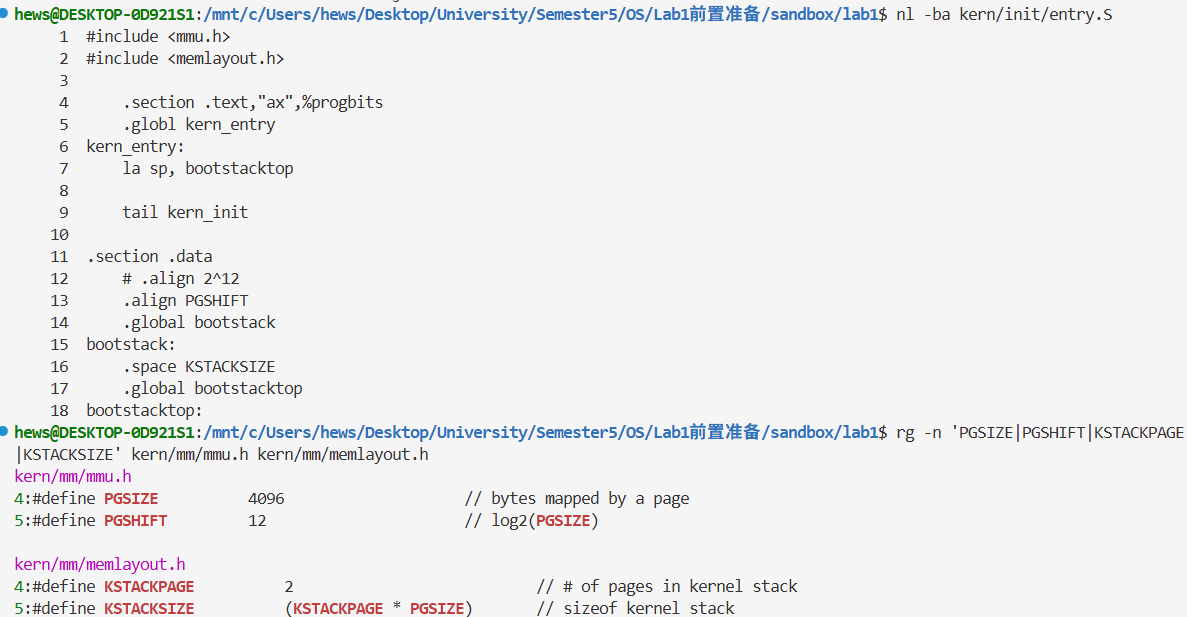
\includegraphics[width=0.9\textwidth]{exercise1-1.png}
    \caption{入口源码、启动栈定义与相关宏}
\end{figure}

这样做的原因是：OpenSBI 交接时 \texttt{sp} 仍指向固件自己的栈（实测为
\texttt{0x80045e30}），这块内存属于固件，内核不能继续使用。而后面马上要进入 C 函数，
C 代码保存返回地址、存放局部变量都离不开栈，所以必须先给内核一个自己的栈。

反汇编显示 \texttt{la} 被展开为两条指令：
\begin{verbatim}
0x80200000 <kern_entry>:    auipc sp,0x3
0x80200004 <kern_entry+4>:  mv    sp,sp
\end{verbatim}
\texttt{auipc} 得到 $\texttt{0x80200000} + \texttt{0x3000} = \texttt{0x80203000}$；
第二条原本是 \texttt{addi sp,sp,0}，因为低 12 位偏移为 0，反汇编显示成了 \texttt{mv}。
用 PC 相对寻址计算地址，意味着这段代码不依赖于绝对地址的硬编码。
\begin{figure}[H]
    \centering
    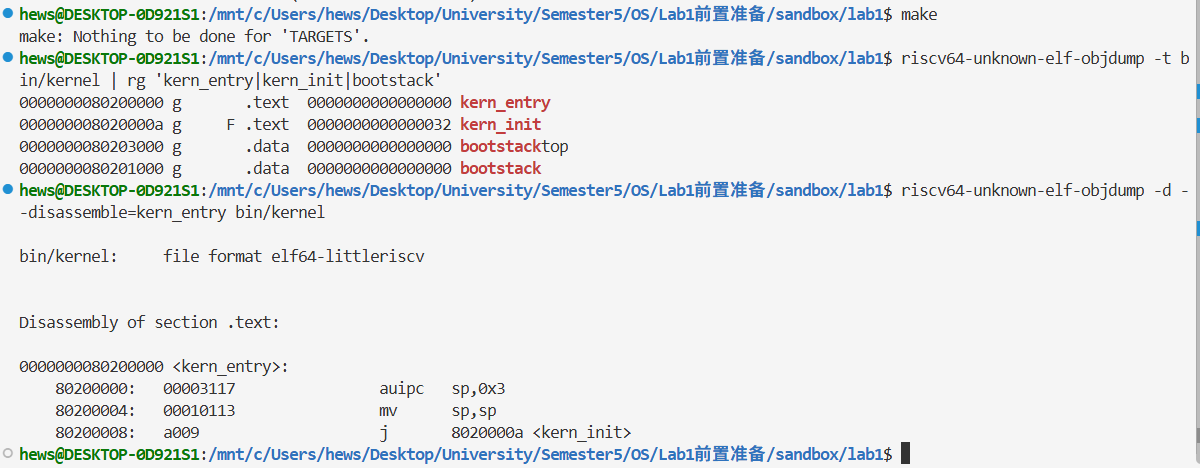
\includegraphics[width=0.9\textwidth]{exercise1-2.png}
    \caption{ELF 符号与 \texttt{kern\_entry} 反汇编}
\end{figure}

\subsubsection{\texttt{tail kern\_init} 的操作与目的}

\texttt{tail} 是尾调用伪指令，效果是跳转到 \texttt{kern\_init}，但不把返回地址写进
\texttt{ra}（展开形式为 \texttt{auipc t1, ...} 加 \texttt{jr t1}，用的是 \texttt{t1}）。
本次链接器做了松弛优化，目标距离很近，最终只剩一条压缩跳转
\texttt{j 0x8020000a}。

不用 \texttt{call} 的原因是 \texttt{kern\_entry} 后面没有任何代码需要执行，
\texttt{kern\_init} 也不会返回。用 \texttt{call} 会写入一个永远用不上的返回地址，
\texttt{tail} 则把控制权直接交出去。

\subsubsection{GDB 验证}
在 \texttt{kern\_entry} 设硬件断点，分别在入口处、执行完 \texttt{la} 对应的两条指令后、
执行完跳转后查看寄存器，结果如下：

\begin{table}[H]
    \centering
    \begin{tabular}{|c|c|c|c|}
        \hline
        时刻 & PC & SP & RA \\
        \hline
        入口指令执行前 & \texttt{0x80200000} & \texttt{0x80045e30} & \texttt{0x80005b52} \\
        \texttt{stepi 2} 之后 & \texttt{0x80200008} & \texttt{0x80203000} & \texttt{0x80005b52} \\
        再 \texttt{stepi} 一次 & \texttt{0x8020000a} & \texttt{0x80203000} & \texttt{0x80005b52} \\
        \hline
    \end{tabular}
\end{table}

\texttt{p \$sp == (unsigned long)\&bootstacktop} 结果为 1，说明栈已设到栈顶；
跳转后 PC 等于 \texttt{\&kern\_init}，而 RA 与入口时相同，说明 \texttt{tail} 确实没有改写
\texttt{ra}。GDB 在 SP 旁边标注 \texttt{<SBI\_CONSOLE\_PUTCHAR>}，是因为这个全局变量在
\texttt{.sdata} 中紧跟启动栈，地址恰好也是 \texttt{0x80203000}，并不代表栈设错了。
\begin{figure}[H]
    \centering
    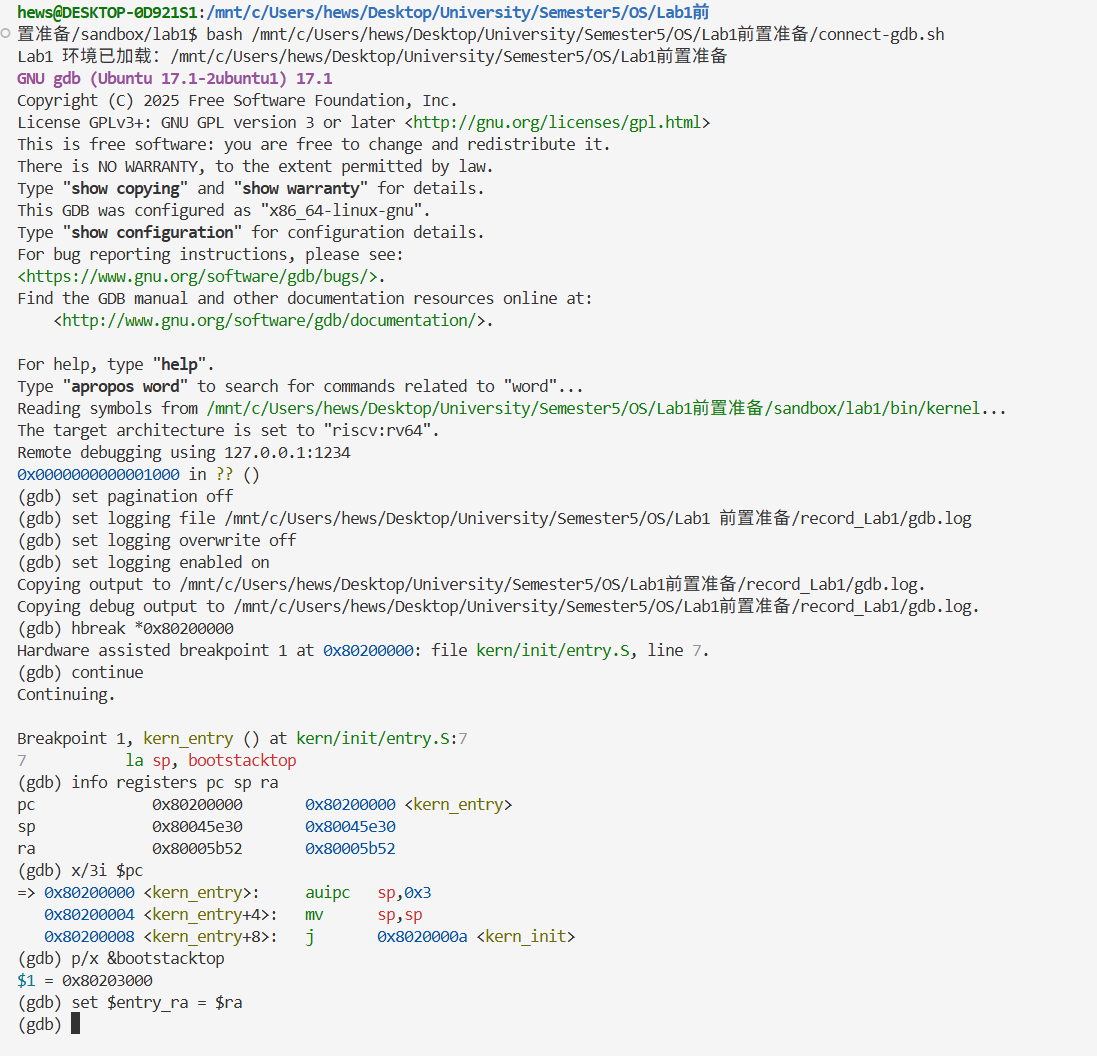
\includegraphics[width=0.75\textwidth]{exercise1-3.png}
    \caption{命中 \texttt{kern\_entry} 断点时的寄存器}
\end{figure}
\begin{figure}[H]
    \centering
    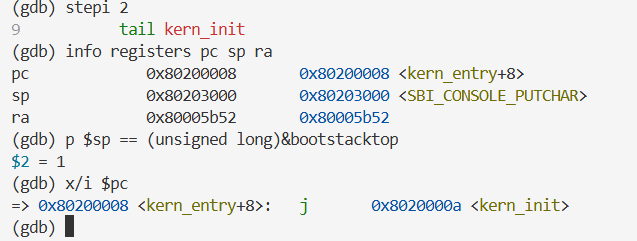
\includegraphics[width=0.7\textwidth]{exercise1-4.png}
    \caption{执行 \texttt{la} 对应的两条指令后，SP 等于 \texttt{bootstacktop}}
\end{figure}
\begin{figure}[H]
    \centering
    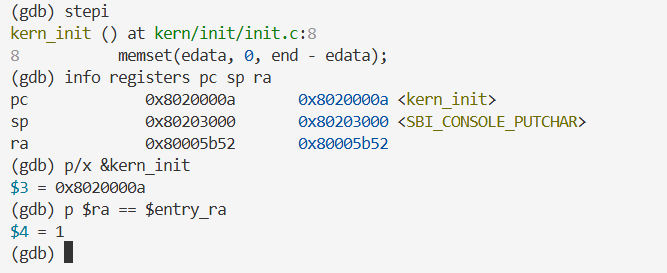
\includegraphics[width=0.72\textwidth]{exercise1-5.png}
    \caption{尾跳转后 PC 到达 \texttt{kern\_init}，RA 不变}
\end{figure}
完整的 GDB 输出见 \path{record_Lab1/logs/gdb.log}。

\subsection{练习二：使用 GDB 验证启动流程}
\textbf{负责人：}陈彦兴、何闻硕

一个终端启动 QEMU 并让 CPU 暂停在复位状态，另一个终端用 GDB 连接\cite{qemu-gdb}，
具体命令见第 \ref{sec:repro} 节。下面按执行顺序列出观察结果，较长的输出只保留相关部分。

\subsubsection{复位地址与最初六条指令}
\begin{verbatim}
(gdb) x/10i 0x1000
   0x1000: auipc t0,0x0
=> 0x1004: addi  a2,t0,40
   0x1008: csrr  a0,mhartid
   0x100c: ld    a1,32(t0)
   0x1010: ld    t0,24(t0)
   0x1014: jr    t0
(gdb) x/2gx 0x1018
0x1018: 0x0000000080000000  0x0000000087e00000
\end{verbatim}
这段输出采集时第一条已经执行，PC 停在 \texttt{0x1004}；重新启动 QEMU 后连接，
PC 为 \texttt{0x1000}、SP 为 0，即复位地址就是 \texttt{0x1000}。各指令的作用：

\begin{table}[H]
    \centering
    \begin{tabular}{|c|c|l|}
        \hline
        地址 & 指令 & 作用 \\
        \hline
        \texttt{0x1000} & \texttt{auipc t0,0x0} & \texttt{t0} = 当前 PC = \texttt{0x1000} \\
        \texttt{0x1004} & \texttt{addi a2,t0,40} & \texttt{a2} = \texttt{0x1028}，启动信息结构的地址 \\
        \texttt{0x1008} & \texttt{csrr a0,mhartid} & \texttt{a0} = 当前 hart 编号，本次为 0 \\
        \texttt{0x100c} & \texttt{ld a1,32(t0)} & 从 \texttt{0x1020} 读出设备树地址 \texttt{0x87e00000} \\
        \texttt{0x1010} & \texttt{ld t0,24(t0)} & 从 \texttt{0x1018} 读出固件入口 \texttt{0x80000000} \\
        \texttt{0x1014} & \texttt{jr t0} & 跳转到 OpenSBI \\
        \hline
    \end{tabular}
\end{table}

\texttt{0x1018} 之后存放的是数据。若继续用 \texttt{x/i} 反汇编，会出现 \texttt{unimp}
之类的指令，那是把数据当成指令解码的结果，CPU 不会执行到这里。
这段复位代码和后面的数据都由 QEMU 生成\cite{qemu-boot}。\texttt{0x1028} 起是交给固件的
启动信息，读出的前两个双字为 \texttt{0x4942534f}（ASCII 为 \texttt{OSBI}）和版本号 2。
\begin{figure}[H]
    \centering
    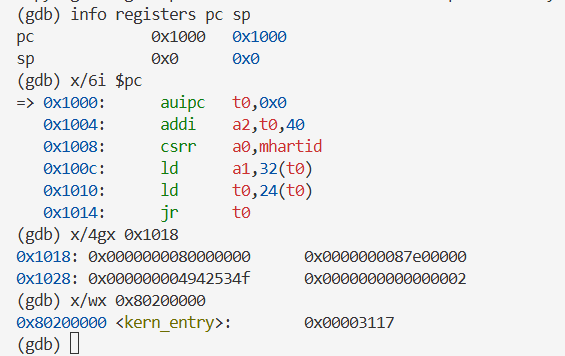
\includegraphics[width=0.65\textwidth]{exercise2-1.png}
    \caption{复位时的 PC/SP、六条复位指令、跳板数据与运行前的内核入口字}
\end{figure}

\subsubsection{进入 OpenSBI}
\texttt{stepi 5} 停在 \texttt{jr t0} 之前，此时 \texttt{t0=0x80000000}、\texttt{a0=0}、
\texttt{a1=0x87e00000}、\texttt{a2=0x1028}（图 \ref{fig:e22}）。再单步一次，PC 变为 \texttt{0x80000000}，
寄存器的相关部分：
\begin{verbatim}
ra             0x0          0x0
sp             0x0          0x0
t0             0x80000000   2147483648
a0             0x0          0
a1             0x87e00000   2279604224
a2             0x1028       4136
pc             0x80000000   0x80000000
\end{verbatim}
参数与复位代码准备的一致，\texttt{sp} 仍为 0，任何栈都还没有建立。
固件入口处的反汇编（节选）：
\begin{verbatim}
(gdb) x/30i 0x80000000
   0x80000000: add s0,a0,zero
   0x80000004: add s1,a1,zero
   0x80000008: add s2,a2,zero
   0x8000000c: jal 0x80000678
   0x80000010: add a6,a0,zero
   0x80000014: add a0,s0,zero
   0x80000018: add a1,s1,zero
   0x8000001c: add a2,s2,zero
   ...
\end{verbatim}
OpenSBI 先把三个参数存到 \texttt{s0}--\texttt{s2}，调用内部函数后再恢复。
这是固件代码，和实验中的 \texttt{entry.S} 无关。固件的初始化过程较长，没有逐条单步。
\begin{figure}[H]
    \centering
    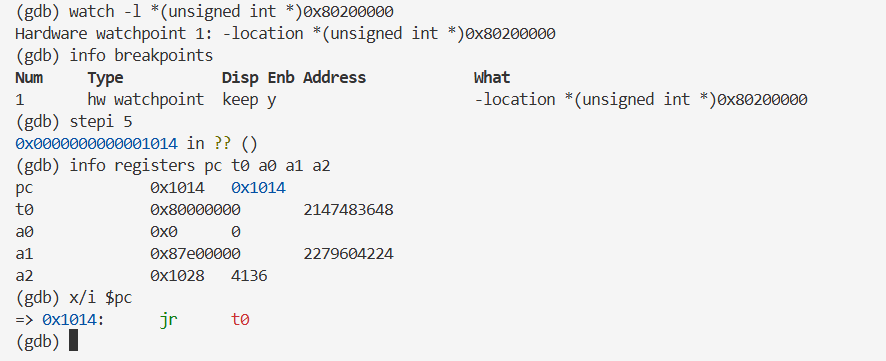
\includegraphics[width=0.85\textwidth]{exercise2-2.png}
    \caption{设置观察点、执行 \texttt{stepi 5} 后 \texttt{jr t0} 前的参数}
    \label{fig:e22}
\end{figure}
\begin{figure}[H]
    \centering
    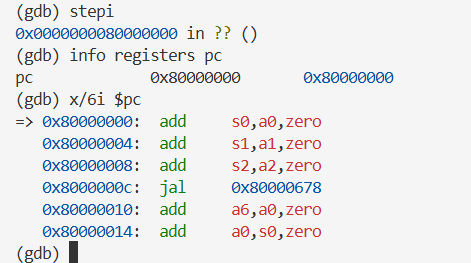
\includegraphics[width=0.55\textwidth]{exercise2-3.png}
    \caption{执行 \texttt{jr t0} 后进入 OpenSBI 第一条指令}
\end{figure}

\subsubsection{OpenSBI 通过 \texttt{mret} 交出控制权}
为了找到固件交接的位置，在固件的 \texttt{mret} 指令（本次固件中位于 \texttt{0x80005b7a}）
设条件硬件断点 \texttt{hbreak *0x80005b7a if \$mepc == 0x80200000}，
同时在 \texttt{0x80200000} 设硬件断点。继续运行后停在 \texttt{mret} 处：
\begin{verbatim}
pc       0x80005b7a
mepc     0x80200000
mstatus  0x8000000a00006800   ... MPP:1 ...
sp       0x80045e30
=> 0x80005b7a:  mret
(gdb) p/x ($mstatus >> 11) & 3
$1 = 0x1
\end{verbatim}
\texttt{mepc} 已设为内核入口，\texttt{mstatus.MPP} 为 1，即 S 模式。\texttt{mret}
执行时，CPU 把特权级切到 MPP 指定的模式，并把 PC 设为 \texttt{mepc}\cite{riscv-priv}。
\begin{figure}[H]
    \centering
    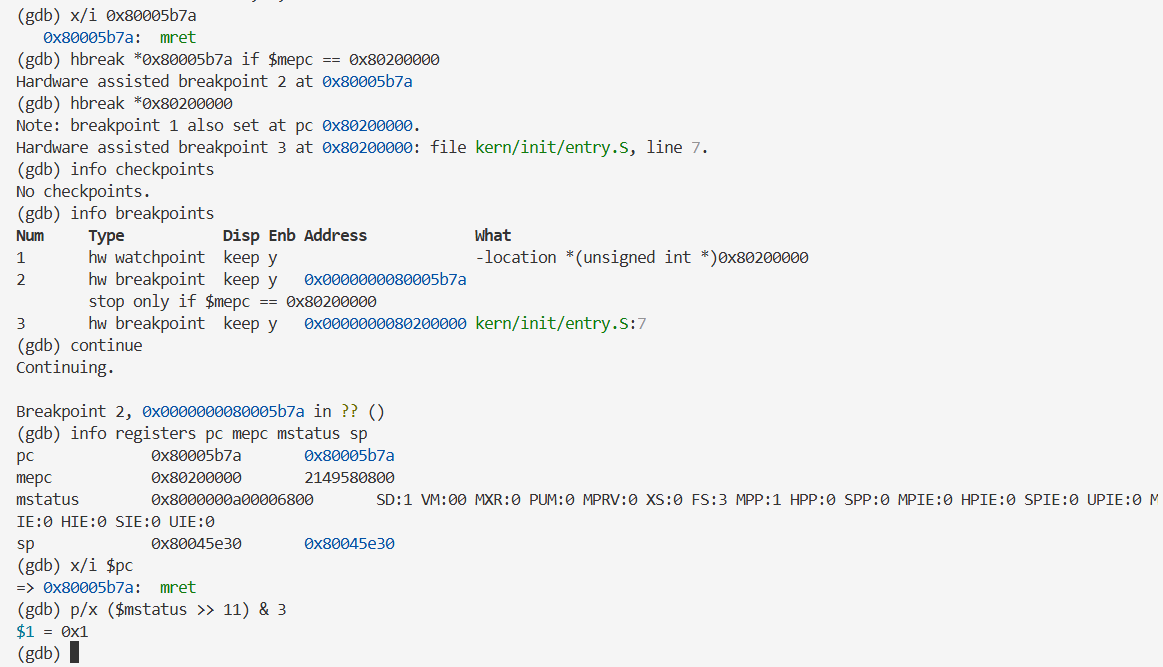
\includegraphics[width=0.9\textwidth]{exercise2-4.png}
    \caption{固件执行 \texttt{mret} 前的 \texttt{mepc}、\texttt{mstatus} 与 MPP 字段}
\end{figure}
OpenSBI 的串口输出中，\texttt{Domain0 Next Address} 为 \texttt{0x80200000}，
\texttt{Domain0 Next Mode} 为 \texttt{S-mode}，与寄存器观察一致。
\begin{figure}[H]
    \centering
    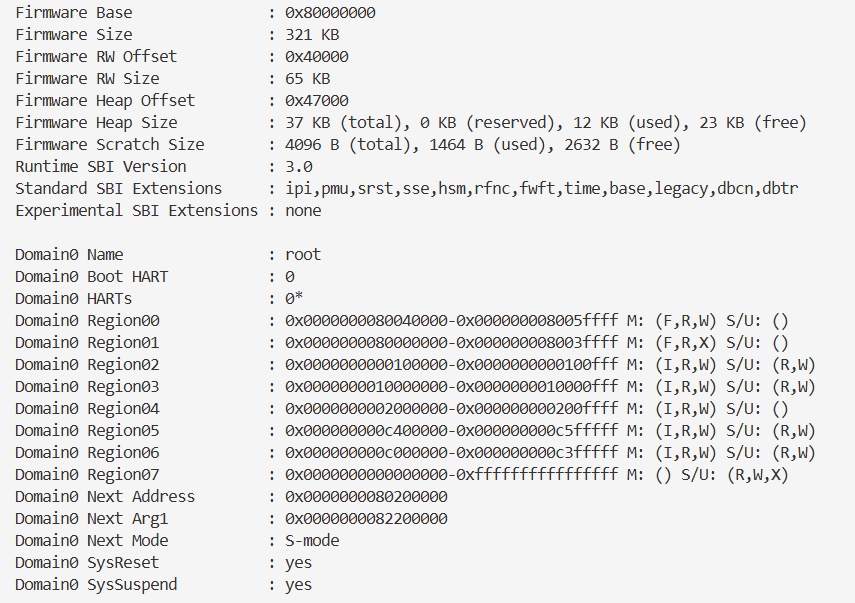
\includegraphics[width=0.75\textwidth]{exercise2-6.png}
    \caption{OpenSBI 输出的固件基址与下一阶段地址、模式}
\end{figure}
图中 \texttt{Next Arg1} 为 \texttt{0x82200000}，而复位阶段 \texttt{a1} 是
\texttt{0x87e00000}。两者属于不同阶段：前者是固件准备交给内核的设备树地址，
FW\_JUMP 固件可以配置这个位置\cite{opensbi-fwjump}。我们只记录了两个阶段的实际值，
没有进一步跟踪设备树的复制过程。

\subsubsection{到达内核入口}
\begin{verbatim}
(gdb) x/10i $pc
=> 0x80200000 <kern_entry>:    auipc sp,0x3
   0x80200004 <kern_entry+4>:  mv    sp,sp
   0x80200008 <kern_entry+8>:  j     0x8020000a <kern_init>
   0x8020000a <kern_init>:     auipc a0,0x3
   0x8020000e <kern_init+4>:   addi  a0,a0,-2
   0x80200012 <kern_init+8>:   auipc a2,0x3
   0x80200016 <kern_init+12>:  addi  a2,a2,-10
   0x8020001a <kern_init+16>:  addi  sp,sp,-16
   0x8020001c <kern_init+18>:  li    a1,0
   0x8020001e <kern_init+20>:  sub   a2,a2,a0
\end{verbatim}
单步执行 \texttt{mret} 后 PC 为 \texttt{0x80200000}，箭头指向内核第一条指令，
它还没有执行。这时 \texttt{sp} 仍是固件栈 \texttt{0x80045e30}，与练习一的观察一致。
\begin{figure}[H]
    \centering
    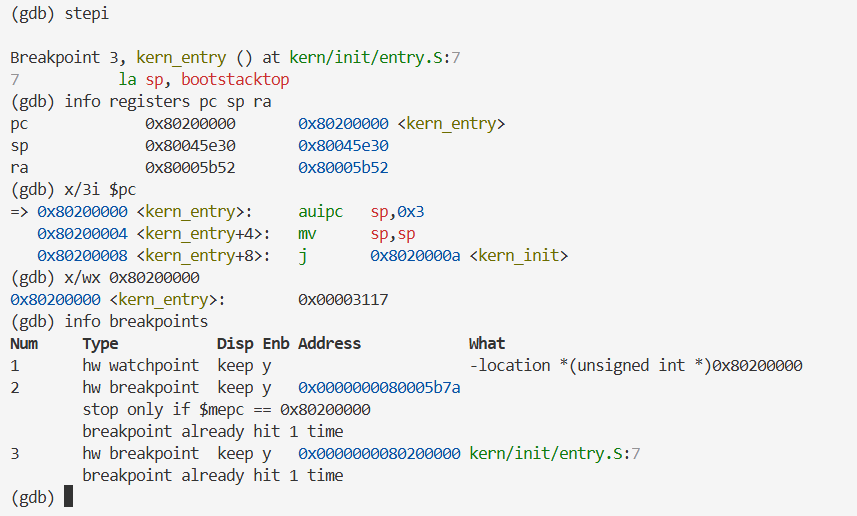
\includegraphics[width=0.8\textwidth]{exercise2-5.png}
    \caption{\texttt{mret} 后到达内核入口，入口指令字与断点命中统计}
\end{figure}

另外，在 CPU 还停在 \texttt{0x1000} 时，\texttt{x/wx 0x80200000} 就已经读到
\texttt{0x00003117}（即 \texttt{auipc sp,0x3} 的编码）。我们对这 4 字节设了
观察点，整个启动过程中它没有被触发。这说明镜像在 CPU 开始执行前已由 QEMU loader
放好，OpenSBI 没有改动入口处的内容。观察点只覆盖这 4 字节，而且只在值变化时触发，
所以这个结论只针对入口指令本身\cite{gdb-watch}。

指导书\cite{lab-guide}的提示认为内核由 SBI 加载到 \texttt{0x80200000}，并建议用
\texttt{watch *0x80200000} 观察加载瞬间。这适用于由固件搬运内核的配置。
本实验的 Makefile 用 \texttt{-device loader} 让 QEMU 在 CPU 运行前写入镜像\cite{qemu-loader}，
所以观察点没有可捕获的变化。我们改用 \texttt{mret} 处的条件断点和
\texttt{0x80200000} 处的断点来确认交接时刻。
练习二的完整 GDB 输出见 \path{record_Lab1/logs/exercise2-reset-gdb.log}。

\subsubsection{问题回答}
RISC-V 硬件加电后最先执行的指令位于 \texttt{0x1000}--\texttt{0x1014}，共 6 条，
由 QEMU 生成。它们的功能是：读取 hart ID 放入 \texttt{a0}，把设备树地址放入
\texttt{a1}，把启动信息地址放入 \texttt{a2}，从紧跟其后的数据区读出固件入口地址
\texttt{0x80000000} 并跳转过去。之后 OpenSBI 在 M 模式下初始化，设置
\texttt{mepc=0x80200000}、\texttt{MPP=S}，通过 \texttt{mret} 进入内核第一条指令。

\subsection{补充观察：内核初始化、输出与死循环}
\subsubsection{BSS 清零的参数}
上面 \texttt{kern\_init} 的反汇编中，\texttt{a0} 由 $\texttt{0x8020000a} + \texttt{0x3000} - 2$
得到 \texttt{0x80203008}，即 \texttt{edata}；\texttt{a2} 由
$\texttt{0x80200012} + \texttt{0x3000} - 10$ 得到同一个地址，即 \texttt{end}；
\texttt{a1} 为 0。\texttt{sub a2,a2,a0} 之后长度为 0，所以这次
\texttt{memset(edata, 0, end - edata)} 实际上什么也没清。原因是当前程序的全局变量
（如 \texttt{SBI\_CONSOLE\_PUTCHAR} 等）都有初值，放在 \texttt{.sdata} 里，\texttt{.bss} 是空的。

\subsubsection{格式化输出调用}
\begin{verbatim}
0x0000000080200036 <+44>: 01e000ef jal 0x80200054 <cprintf>
0x000000008020003a <+48>: a001     j   0x8020003a <kern_init+48>
\end{verbatim}
\texttt{jal} 调用 \texttt{cprintf}，返回地址 \texttt{0x8020003a} 写入 \texttt{ra}。
字符串由 \texttt{cprintf} 及其下层函数输出；第二条是跳转到自身的指令，
就是源码中的 \texttt{while (1);}。

\subsubsection{在 OpenSBI 中无法回溯}
\begin{verbatim}
(gdb) finish
"finish" not meaningful in the outermost frame.
(gdb) bt
#0  0x000000008000caae in ?? ()
\end{verbatim}
跟踪字符输出时，PC 进入了 OpenSBI 的地址范围（\texttt{ecall} 之后由固件处理）。GDB 只加载了内核的符号，
不认识固件代码，也就无法展开调用栈，于是把当前帧当成了最外层，\texttt{finish} 报错。
这个提示只是 GDB 缺少调试信息，并不说明程序真的处在最外层函数。
要回到内核，可以在 \texttt{0x8020003a} 设断点后 \texttt{continue}。

\subsubsection{输出完成后的执行位置}
\begin{verbatim}
(gdb) x/10i $pc
=> 0x8020003a <kern_init+48>: j     0x8020003a <kern_init+48>
   0x8020003c <cputch>:      addi  sp,sp,-32
   0x8020003e <cputch+2>:    sd    ra,24(sp)
   0x80200040 <cputch+4>:    sd    a1,8(sp)
   0x80200042 <cputch+6>:    jal   0x80200088 <cons_putc>
   ...
\end{verbatim}
输出结束后 PC 停在跳转到自身的指令上。后面的 \texttt{cputch} 只是在内存中恰好相邻的
另一个函数，\texttt{x/10i} 连续反汇编时被一并显示出来，CPU 并不会顺序执行到那里。

\subsection{AI 辅助学习与调试过程}
本实验没有编写或修改内核代码，因此不涉及功能实现的提示词和代码迭代。
AI 主要用在三个方面：解释 \texttt{la}、\texttt{tail}、\texttt{mret} 等指令和
OpenSBI 的交接机制；根据我们贴出的 GDB 输出帮忙分析现象；整理实验记录和报告文字。

下面几处是借助 AI 理解时容易出错、后来对照源码和 GDB 结果才确认的地方：
\begin{itemize}
    \item 启动栈的位置。容易误以为启动栈在 \texttt{0x80000000} 附近。
          查看链接脚本和 \texttt{nm} 输出后确认，启动栈在内核 \texttt{.data} 段中，
          地址为 \texttt{0x80201000}--\texttt{0x80203000}，\texttt{0x80000000} 是 OpenSBI 的位置。
    \item \texttt{0x1018} 之后的 \texttt{unimp}。反汇编输出容易被理解为复位代码的一部分，
          用 \texttt{x/2gx} 按数据查看后才确认那里存的是两个地址。
    \item \texttt{finish} 的报错。报错信息字面上说处于最外层帧，实际是 GDB 没有固件符号，
          不能据此推断程序的调用关系。
    \item SP 旁的 \texttt{<SBI\_CONSOLE\_PUTCHAR>} 标注。对照符号表后确认只是地址重合。
\end{itemize}
报告中的地址和寄存器值全部取自实际 GDB 输出和本次构建的符号表，没有使用 AI 推算的数值。

\section{测试与验证}
\subsection{编译与运行结果}
在仓库根目录执行 \texttt{make -C lab1 clean} 后重新 \texttt{make -C lab1}，
各源文件依次编译，最后链接出 \texttt{bin/kernel} 并用 \texttt{objcopy} 生成
\texttt{bin/ucore.img}，命令退出码为 0：
\begin{verbatim}
+ cc libs/sbi.c
+ cc libs/string.c
+ ld bin/kernel
riscv64-unknown-elf-objcopy bin/kernel --strip-all -O binary bin/ucore.img
\end{verbatim}
用与 \texttt{make qemu} 相同的参数运行 QEMU，控制台输出（节选）：
\begin{verbatim}
OpenSBI v1.8.1
Platform Name               : riscv-virtio,qemu
Firmware Base               : 0x80000000
Runtime SBI Version         : 3.0
Domain0 Next Address        : 0x0000000080200000
Domain0 Next Mode           : S-mode
(THU.CST) os is loading ...
\end{verbatim}
内核横幅正常输出。下图是调试过程中的截图，左侧为 QEMU 控制台，右侧为 GDB 会话，
在 GDB 中 \texttt{continue} 之后左侧出现了内核输出。
\begin{figure}[H]
    \centering
    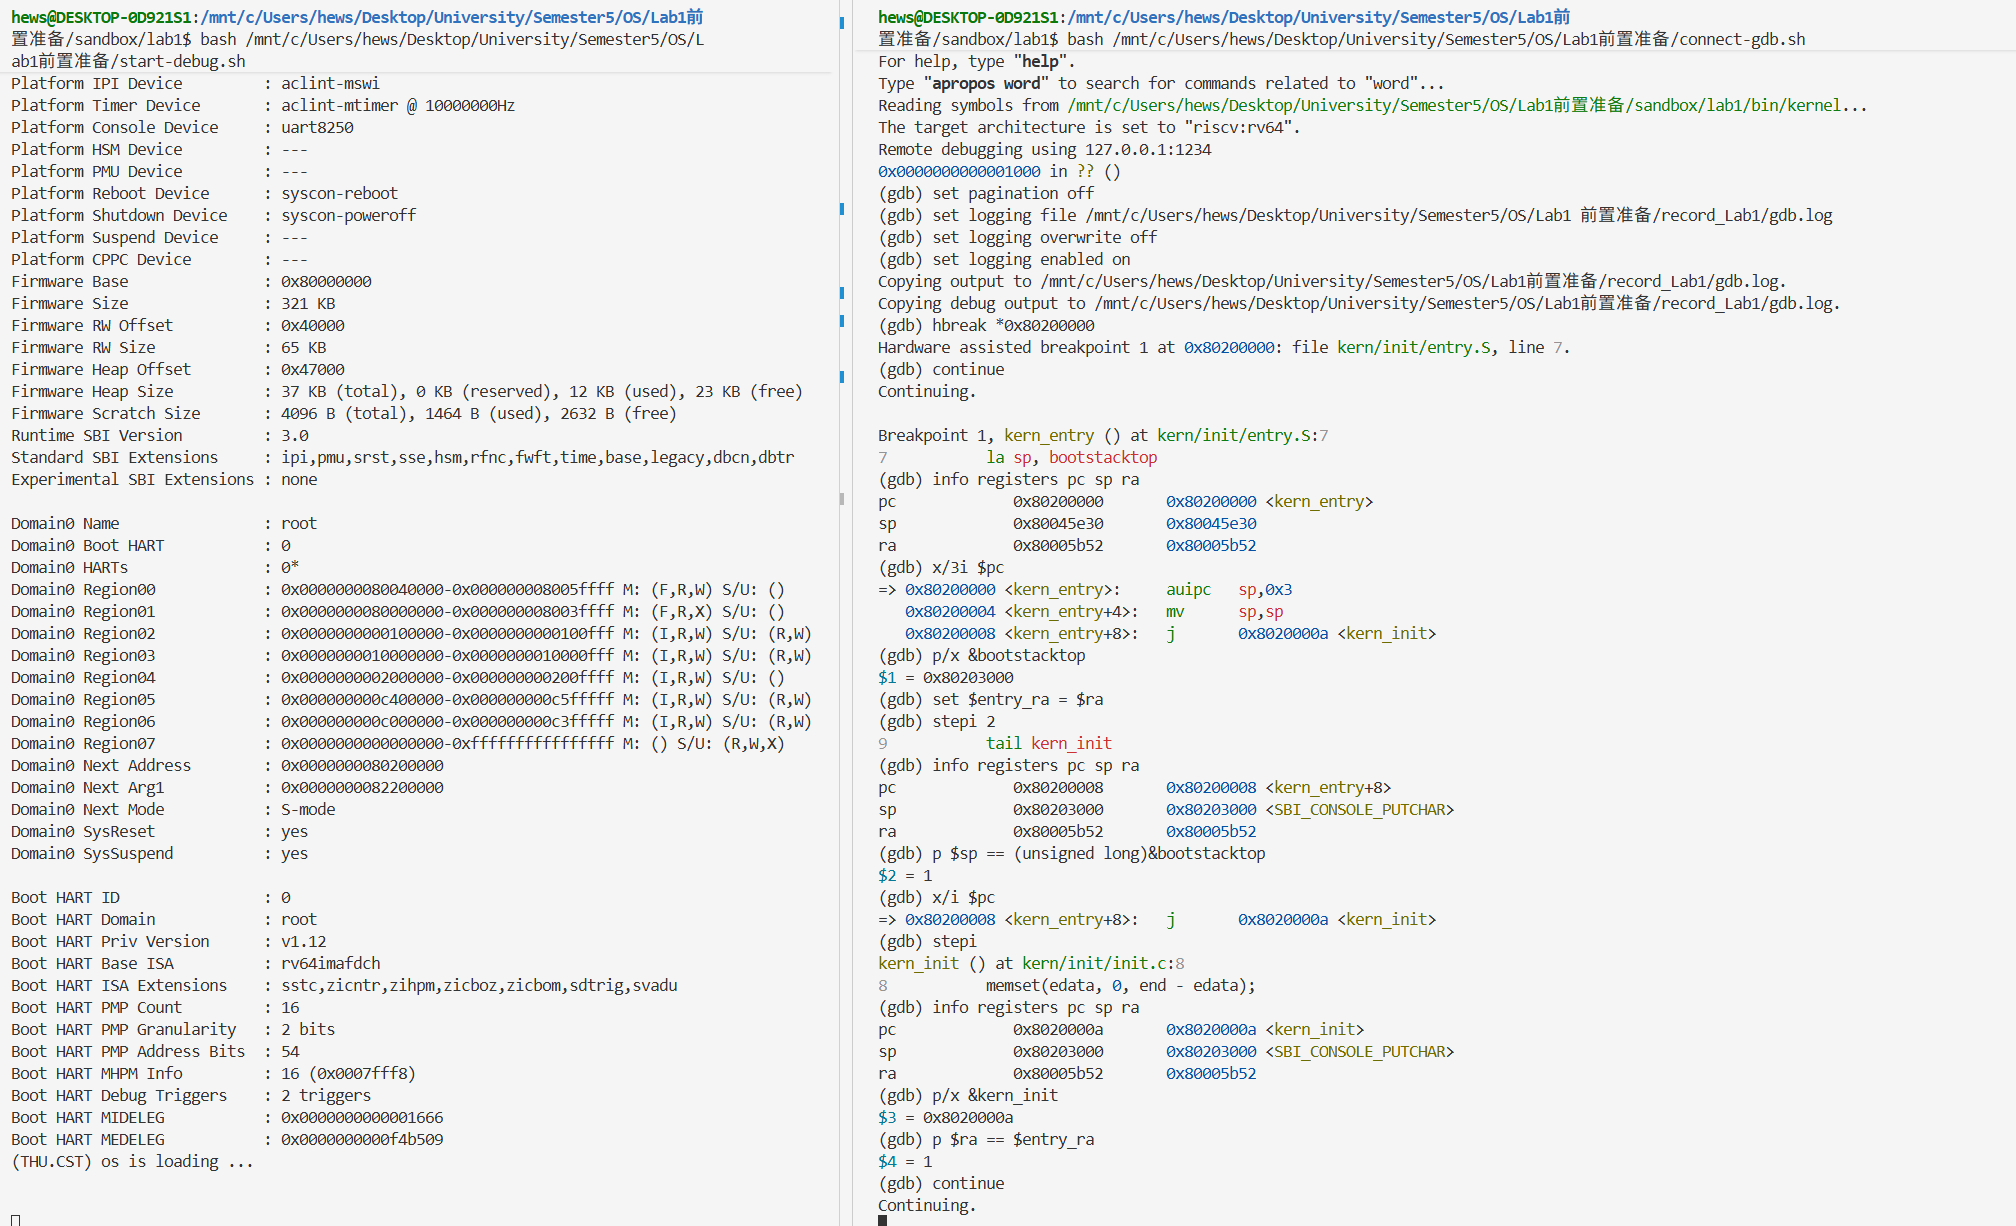
\includegraphics[width=\textwidth]{exercise1-6.png}
    \caption{QEMU 控制台输出与 GDB 调试过程}
\end{figure}

\subsection{启动流程的 GDB 验证结果}
\begin{table}[H]
    \centering
    \begin{tabular}{|c|c|c|l|}
        \hline
        阶段 & PC & SP & 依据 \\
        \hline
        复位 & \texttt{0x1000} & \texttt{0x0} & 新启动 QEMU 后连接 GDB \\
        进入 OpenSBI & \texttt{0x80000000} & \texttt{0x0} & \texttt{jr t0} 后单步 \\
        固件交接前 & \texttt{0x80005b7a} & \texttt{0x80045e30} & \texttt{mepc=0x80200000}，\texttt{MPP=1} \\
        内核入口 & \texttt{0x80200000} & \texttt{0x80045e30} & \texttt{mret} 后命中断点 \\
        栈设置后 & \texttt{0x80200008} & \texttt{0x80203000} & 等于 \texttt{\&bootstacktop} \\
        进入 C 代码 & \texttt{0x8020000a} & \texttt{0x80203000} & 等于 \texttt{\&kern\_init}，RA 不变 \\
        输出完成 & \texttt{0x8020003a} & -- & 停在 \texttt{while (1)} \\
        \hline
    \end{tabular}
\end{table}

\subsection{复现方法}\label{sec:repro}
以下命令在仓库根目录执行。构建并查看符号与入口反汇编：
\begin{verbatim}
make -C lab1
riscv64-unknown-elf-objdump -t lab1/bin/kernel \
  | grep -E 'kern_entry|kern_init|bootstack'
riscv64-unknown-elf-objdump -d --disassemble=kern_entry lab1/bin/kernel
\end{verbatim}
终端 A 启动 QEMU 并暂停 CPU（\texttt{fw\_jump.bin} 换成本机实际路径）：
\begin{verbatim}
qemu-system-riscv64 -machine virt -nographic -bios /path/to/fw_jump.bin \
  -device loader,file=lab1/bin/ucore.img,addr=0x80200000 \
  -gdb tcp:127.0.0.1:1234 -S
\end{verbatim}
这里显式指定 FW\_JUMP，与采集截图时的配置一致。新版 QEMU 默认使用的 OpenSBI
可能是 FW\_DYNAMIC 类型，在只用 loader 装入镜像的情况下，不能保证它会跳到 \texttt{0x80200000}。

终端 B 执行 \texttt{riscv64-unknown-elf-gdb lab1/bin/kernel}，然后依次输入：
\begin{verbatim}
set architecture riscv:rv64
target remote 127.0.0.1:1234
info registers pc sp
x/6i $pc
x/4gx 0x1018
x/wx 0x80200000
watch -l *(unsigned int *)0x80200000
stepi 5
info registers pc t0 a0 a1 a2
stepi
x/6i $pc
x/i 0x80005b7a
hbreak *0x80005b7a if $mepc == 0x80200000
hbreak *0x80200000
continue
info registers pc mepc mstatus sp
p/x ($mstatus >> 11) & 3
stepi
info registers pc sp ra
set $entry_ra = $ra
stepi 2
p $sp == (unsigned long)&bootstacktop
stepi
p/x &kern_init
p $ra == $entry_ra
\end{verbatim}
\texttt{0x80005b7a} 是本次固件中 \texttt{mret} 的地址，换固件后要先重新找到交接处的
\texttt{mret}。最后 \texttt{detach}，QEMU 继续运行并输出内核横幅；在终端 A 按
\texttt{Ctrl+A} 后按 \texttt{X} 退出。

\subsection{验证范围与未执行项目}
\begin{itemize}
    \item 已验证：干净编译、QEMU 运行输出，以及从复位到 \texttt{kern\_init} 死循环的完整 GDB 跟踪。
    \item GDB 跟踪是在小组另一台机器上完成的（QEMU 10.2.1，固件为 OpenSBI FW\_JUMP），
          编译与运行结果来自上表所列环境。\texttt{0x80005b7a}、\texttt{0x80045e30} 等固件内部地址
          与固件版本有关，换环境后需要重新定位；内核符号地址由链接脚本决定，两边一致。
    \item 未单步跟踪 OpenSBI 内部的初始化过程，只观察了它的入口和交接点。
    \item 原始截图和日志保存在 \path{doc/lab1/record_Lab1/}，
          \texttt{evidence-manifest.json} 记录了每个文件的大小和 SHA-256，报告中的截图未经裁剪或修改。
    \item 本实验目录中没有评分脚本 \texttt{tools/grade.sh}，未运行 \texttt{make grade}。
\end{itemize}

\section{实验总结与收获}
\subsection{实验知识点与操作系统原理的联系和差异}
\begin{itemize}
    \item \textbf{启动过程}：原理课讲的是 BIOS 加载引导程序、引导程序加载内核。
          本实验对应的是复位代码 $\rightarrow$ OpenSBI $\rightarrow$ 内核，分工类似，
          但内核由 QEMU 直接放入内存，OpenSBI 不负责从磁盘读取内核，这一点和 x86 上
          BIOS + bootloader 读盘的流程不同。
    \item \textbf{特权级}：原理课只区分内核态和用户态。RISC-V 有 M、S、U 三级，
          本实验中固件运行在 M 模式，内核运行在 S 模式，从 M 到 S 的切换通过
          \texttt{mret} 和 \texttt{mstatus.MPP} 完成。
    \item \textbf{系统调用与固件接口}：内核用 \texttt{ecall} 请求 OpenSBI 输出字符，
          形式上和用户程序通过系统调用请求内核服务是一样的，只是发生在 S 到 M 之间。
    \item \textbf{内存布局}：链接脚本决定了内核各段的地址，C 代码需要的栈和清零的 BSS
          都依赖这里导出的符号。原理课中“程序装入内存”的过程在这里要手工写出来。
    \item \textbf{栈与调用约定}：没有栈就不能运行 C 代码，所以入口汇编的第一件事就是设置
          \texttt{sp}。\texttt{tail} 与 \texttt{call} 的区别也来自调用约定中 \texttt{ra} 的用法。
\end{itemize}

\subsection{重要但本实验尚未涉及的操作系统知识点}
本实验的内核没有中断和异常处理，也没有时钟，不能做任何调度；没有页表，
运行在物理地址上，\texttt{satp} 未开启分页；没有物理内存管理和堆分配；
没有进程、线程和用户态程序，也没有文件系统和设备驱动，串口输出完全依赖 OpenSBI。
这些内容会在后续实验中陆续加入。

\subsection{调试中遇到的问题与解决方法}
\begin{itemize}
    \item \textbf{调试会话状态不对}：第一次做练习二时，GDB 连上后 PC 是
          \texttt{0x8020003a}，也就是内核死循环的位置，原因是 QEMU 已经运行过一遍。
          退出旧的 GDB 和 QEMU，重新用 \texttt{-S} 启动后，确认 PC 为 \texttt{0x1000}、
          SP 为 0，再开始记录。排查时的旧日志保留在
          \path{record_Lab1/logs/diagnostics/exercise2-gdb.log}。
    \item \textbf{地址混淆}：\texttt{0x1000}、\texttt{0x80000000}、\texttt{0x80200000}
          和启动栈地址容易混在一起。对照链接脚本、\texttt{nm} 输出和 OpenSBI 的启动信息，
          分别确认它们是复位代码、固件、内核入口和内核数据段中的地址。
    \item \textbf{数据被当作指令}：\texttt{x/i} 连续反汇编会把 \texttt{0x1018} 后面的数据
          显示成指令。改用 \texttt{x/gx} 按 8 字节查看后读出了两个地址。
    \item \textbf{在 OpenSBI 中无法回溯}：PC 进入固件后 \texttt{bt}、\texttt{finish} 都失效。
          GDB 没有固件的符号，只能在内核中的地址（如 \texttt{0x8020003a}）设断点再 \texttt{continue} 回到内核。
\end{itemize}

\subsection{AI 协作经验与个人收获}
AI 在解释指令和梳理启动流程时很省时间，但它给出的具体地址和寄存器值经常是按“一般情况”
推出来的，和本次构建并不一致。我们的做法是：概念可以先听 AI 的解释，
数值一律以 GDB 输出和 \texttt{nm}、\texttt{objdump} 的结果为准，有冲突时回到源码和
链接脚本确认。提问时附上完整的 GDB 输出，比只描述现象更容易得到对得上的解释。

通过这次实验，我们弄清了一个最小内核从上电到打印第一行字之前需要哪些准备：
有人把镜像放进内存，有人把 CPU 切到正确的特权级并跳到入口，入口代码设置好栈，
C 代码才能运行。也熟悉了用 GDB 调试裸机程序的方法，包括硬件断点、条件断点、
观察点以及查看 CSR 寄存器。

%----------------------------------------------------------------
\newpage
\bibliographystyle{plain}
\bibliography{references} 
\end{document}
